\documentclass[12pt, titlepage]{article}

\usepackage{fullpage}
\usepackage[round]{natbib}
\usepackage{multirow}
\usepackage{booktabs}
\usepackage{tabularx}
\usepackage{graphicx}
\usepackage{float}
\usepackage{xr}
\usepackage{hyperref}
\hypersetup{
    colorlinks,
    citecolor=black,
    filecolor=black,
    linkcolor=red,
    urlcolor=blue
}

%% Comments

\usepackage{color}

\newif\ifcomments\commentstrue

\ifcomments
\newcommand{\authornote}[3]{\textcolor{#1}{[#3 ---#2]}}
\newcommand{\todo}[1]{\textcolor{red}{[TODO: #1]}}
\else
\newcommand{\authornote}[3]{}
\newcommand{\todo}[1]{}
\fi

\newcommand{\wss}[1]{\authornote{blue}{SS}{#1}} 
\newcommand{\plt}[1]{\authornote{magenta}{TPLT}{#1}} %For explanation of the template
\newcommand{\an}[1]{\authornote{cyan}{Author}{#1}}

%% Common Parts

\newcommand{\progname}{ProgName} % PUT YOUR PROGRAM NAME HERE %Every program
                                % should have a name


\externaldocument{../MIS/MIS}
\externaldocument[CA-]{../../Commonality-Analysis/CA}

\newcounter{acnum}
\newcommand{\actheacnum}{AC\theacnum}
\newcommand{\acref}[1]{AC\ref{#1}}

\newcounter{ucnum}
\newcommand{\uctheucnum}{UC\theucnum}
\newcommand{\uref}[1]{UC\ref{#1}}

\newcounter{mnum}
\newcommand{\mthemnum}{M\themnum}
\newcommand{\mref}[1]{M\ref{#1}}


\begin{document}

\title{Module Guide for Family of Light Models} 
\author{Sasha Soraine}
\date{\today}

\maketitle

\pagenumbering{roman}

\section{Revision History}

\begin{tabularx}{\textwidth}{p{3cm}p{2cm}X}
\toprule {\bf Date} & {\bf Version} & {\bf Notes}\\
\midrule
Date 1 & 1.0 & Notes\\
Date 2 & 1.1 & Notes\\
\bottomrule
\end{tabularx}

\newpage

\section{Reference Material}

This section records information for easy reference.

\subsection{Abbreviations and Acronyms}

\renewcommand{\arraystretch}{1.2}
\begin{tabular}{l l} 
  \toprule		
  \textbf{symbol} & \textbf{description}\\
  \midrule 
  AC & Anticipated Change\\
  DAG & Directed Acyclic Graph \\
  M & Module \\
  MG & Module Guide \\
  OS & Operating System \\
  R & Requirement\\
  SC & Scientific Computing \\
  SRS & Software Requirements Specification\\
  Lighting Models & Explanation of program name\\
  UC & Unlikely Change \\
  \bottomrule
\end{tabular}\\

\newpage

\tableofcontents

\listoftables

\listoffigures

\newpage

\pagenumbering{arabic}

\section{Introduction}

Decomposing a system into modules is a commonly accepted approach to developing
software.  A module is a work assignment for a programmer or programming
team~\citep{ParnasEtAl1984}.  We advocate a decomposition
based on the principle of information hiding~\citep{Parnas1972a}.  This
principle supports design for change, because the ``secrets'' that each module
hides represent likely future changes.  Design for change is valuable in SC,
where modifications are frequent, especially during initial development as the
solution space is explored.  

Our design follows the rules laid out by \citet{ParnasEtAl1984}, as follows:
\begin{itemize}
\item System details that are likely to change independently should be the
  secrets of separate modules.
\item Each data structure is implemented in only one module.
\item Any other program that requires information stored in a module's data
  structures must obtain it by calling access programs belonging to that module.
\end{itemize}

After completing the first stage of the design, the Software Requirements
Specification (SRS), the Module Guide (MG) is developed~\citep{ParnasEtAl1984}. The MG
specifies the modular structure of the system and is intended to allow both
designers and maintainers to easily identify the parts of the software.  The
potential readers of this document are as follows:

\begin{itemize}
\item New project members: This document can be a guide for a new project member
  to easily understand the overall structure and quickly find the
  relevant modules they are searching for.
\item Maintainers: The hierarchical structure of the module guide improves the
  maintainers' understanding when they need to make changes to the system. It is
  important for a maintainer to update the relevant sections of the document
  after changes have been made.
\item Designers: Once the module guide has been written, it can be used to
  check for consistency, feasibility and flexibility. Designers can verify the
  system in various ways, such as consistency among modules, feasibility of the
  decomposition, and flexibility of the design.
\end{itemize}

The rest of the document is organized as follows. Section
\ref{SecChange} lists the anticipated and unlikely changes of the software
requirements. Section \ref{SecMH} summarizes the module decomposition that
was constructed according to the likely changes. Section \ref{SecConnection}
specifies the connections between the software requirements and the
modules. Section \ref{SecMD} gives a detailed description of the
modules. Section \ref{SecTM} includes two traceability matrices. One checks
the completeness of the design against the requirements provided in the SRS. The
other shows the relation between anticipated changes and the modules. Section
\ref{SecUse} describes the use relation between modules.

\section{Anticipated and Unlikely Changes} \label{SecChange}

This section lists possible changes to the system. According to the likeliness
of the change, the possible changes are classified into two
categories. Anticipated changes are listed in Section \ref{SecAchange}, and
unlikely changes are listed in Section \ref{SecUchange}.

\subsection{Anticipated Changes} \label{SecAchange}

Anticipated changes are the source of the information that is to be hidden
inside the modules. Ideally, changing one of the anticipated changes will only
require changing the one module that hides the associated decision. The approach
adapted here is called design for
change.

\begin{description}
\item[\refstepcounter{acnum} \actheacnum \label{acHardware}:] The specific
  hardware on which the software is running.
\item[\refstepcounter{acnum} \actheacnum \label{acInput}:] The format of the
  initial input data.
\item[\refstepcounter{acnum} \actheacnum \label{acOutput}:] The format of the
output data.
\item[\refstepcounter{acnum} \actheacnum \label{acNormalCalculation}:] The 
algorithm for calculating surface normals. %%The algorithm may change, or there 
%%might not be one if the input changes to include a normal map.
\item[\refstepcounter{acnum} \actheacnum \label{acNormalInterpolation}:] The 
algorithm for interpolating surface normals.
\item[\refstepcounter{acnum} \actheacnum \label{acLightingModels}:] The 
algorithm for calculating the final colouring of objects. %%The algorithm may 
%%change, or there might not be one if the input changes to include a normal 
%%map.
\item[\refstepcounter{acnum} \actheacnum \label{acShapes}:] The 
format for representing object shapes. 
\item[\refstepcounter{acnum} \actheacnum \label{acLights}:] The 
format for representing light sources. 

\end{description}

\subsection{Unlikely Changes} \label{SecUchange}
The module design should be as general as possible. However, a general system is
more complex. Sometimes this complexity is not necessary. Fixing some design
decisions at the system architecture stage can simplify the software design. If
these decision should later need to be changed, then many parts of the design
will potentially need to be modified. Hence, it is not intended that these
decisions will be changed.

\begin{description}
\item[\refstepcounter{ucnum} \uctheucnum \label{ucIO}:] Input/Output devices
  (Input: File and/or Keyboard, Output: File, Memory, and/or Screen).
\item[\refstepcounter{ucnum} \uctheucnum \label{ucCartesian}:] The format of 3D 
coordinates and vectors.

\end{description}

\section{Module Hierarchy} \label{SecMH}

This section provides an overview of the module design. Modules are summarized
in a hierarchy decomposed by secrets in Table \ref{TblMH}. The modules listed
below, which are leaves in the hierarchy tree, are the modules that will
actually be implemented.

\begin{description}
\item [\refstepcounter{mnum} \mthemnum \label{mHH}:] Hardware-Hiding Module
\item [\refstepcounter{mnum} \mthemnum \label{mInputs}:] Input Parameters Module
\item [\refstepcounter{mnum} \mthemnum \label{mOutputs}:] Output Format Module
\item [\refstepcounter{mnum} \mthemnum \label{mPolygon}:] Polygon Module
\item [\refstepcounter{mnum} \mthemnum \label{mColour}:] Colour Module
\item [\refstepcounter{mnum} \mthemnum \label{mPoints}:] 3D Cartesian 
Coordinate 
Module
\item [\refstepcounter{mnum} \mthemnum \label{mTypes}:] Light Types 
Module
\item [\refstepcounter{mnum} \mthemnum \label{mMesh}:] Polygon Mesh Module
\item [\refstepcounter{mnum} \mthemnum \label{mNormals}:] Normal Map Module
\item [\refstepcounter{mnum} \mthemnum \label{mScene}:] Scene Module
\item [\refstepcounter{mnum} \mthemnum \label{mObjects}:] Object Module
\item [\refstepcounter{mnum} \mthemnum \label{mLights}:] Light Source Module
\item [\refstepcounter{mnum} \mthemnum \label{mObsv}:] Observer Module
\item [\refstepcounter{mnum} \mthemnum \label{mVectors}:] Vector Module
\item [\refstepcounter{mnum} \mthemnum \label{mVecMath}:] Vector Math Module
\item [\refstepcounter{mnum} \mthemnum \label{mShader}:] Shader Module
\item [\refstepcounter{mnum} \mthemnum \label{mLightModel}:] Lighting Model 
Module
\item [\refstepcounter{mnum} \mthemnum \label{mJSON}:] JSON Module
\item [\refstepcounter{mnum} \mthemnum \label{mUnity}:] Rendering Module
\end{description}


\begin{table}[h!]
\centering
\begin{tabular}{p{0.3\textwidth} p{0.6\textwidth}}
\toprule
\textbf{Level 1} & \textbf{Level 2}\\
\midrule

{Hardware-Hiding Module} & ~ \\
\midrule

\multirow{8}{0.3\textwidth}{Behaviour-Hiding Module} & Input Parameters Module\\
%%Purpose of the input parameters module is to parse the JSON file and separate 
%%it into usable objects
& Output Format Module \\
%% Purpose is to create the output of the module
& Polygon Module\\
& Colour Module\\
& 3D Cartesian Coordinate Module\\ %%Data type for representing cartesian 
%%coordinates; works with the vector math module to define vectors and 
%%calculate 
%%things
& Light Type Module \\
& Polygon Mesh Module\\ %I'm not reinventing the wheel with this module; people 
%smarter than me have implemented polygon mesh libraries and data structures.
& Normal Maps Module\\ %I'm not reinventing the wheel with this module; people 
%smarter than me have implemented vector calculus.
& Scene Module\\
%% Data type definition of a scene in this program
& Object Module\\
%% Data type definition of an object in this program
& Light Source Module\\
%% Data type definition of a light source in this program
& Observer Module \\
%% Data type definition of an observer in this program
& Vector Math Module\\ %I'm not reinventing the wheel with this module; people 
%smarter than me have implemented vector calculus.
& Shader Module\\
& Lighting Model Module\\
\midrule
\multirow{2}{0.3\textwidth}{Software Decision Module} 
& JSON Module\\ %I need the JSON module to parse and write JSON files
& Rendering Module\\ %Rationale: The outputted JSON file will be passed back to 
%unity for rendering
\bottomrule

\end{tabular}
\caption{Module Hierarchy}
\label{TblMH}
\end{table}

\section{Connection Between Requirements and Design} \label{SecConnection}

The design of the system is intended to satisfy the requirements developed in
the SRS. In this stage, the system is decomposed into modules. The connection
between requirements and modules is listed in Table \ref{TblRT}.


%\wss{The intention of this section is to document decisions that are made
%``between'' the requirements and the design.  To satisfy some requirements,
%design decisions need to be made.  Rather than make these decisions implicit,
%they are explicitly recorded here.  For instance, if a program has security
%requirements, a specific design decision may be made to satisfy those
%requirements with a password.  In scientific examples, the choice of algorithm
%could potentially go here, if that is a decision that is exposed by the
%interface.}

%%TO DO:
% - talk about the JSON design decision
% - talk about implementing as a system plug-in for unity to leverage GUI
% - talk about types being used and why

\section{Module Decomposition} \label{SecMD}

Modules are decomposed according to the principle of ``information hiding''
proposed by \citet{ParnasEtAl1984}. The \emph{Secrets} field in a module
decomposition is a brief statement of the design decision hidden by the
module. The \emph{Services} field specifies \emph{what} the module will do
without documenting \emph{how} to do it. For each module, a suggestion for the
implementing software is given under the \emph{Implemented By} title. If the
entry is \emph{OS}, this means that the module is provided by the operating
system or by standard programming language libraries.  \emph{Lighting Models} 
means 
the
module will be implemented by the Lighting Models software.

Only the leaf modules in the hierarchy have to be implemented. If a dash
(\emph{--}) is shown, this means that the module is not a leaf and will not have
to be implemented.

\subsection{Hardware Hiding Modules (\mref{mHH})}
The following section outlines the hardware hiding modules. Their 
descriptions follow the format below: 

\begin{description}
\item[Secrets:]The data structure and algorithm used to implement the virtual
  hardware.
\item[Services:]Serves as a virtual hardware used by the rest of the
  system. This module provides the interface between the hardware and the
  software. So, the system can use it to display outputs or to accept inputs.
\item[Implemented By:] OS
\end{description}

\subsection{Behaviour-Hiding Module}
The following section outlines the behaviour-hiding modules. Their 
descriptions follow the format below: 

\begin{description}
\item[Secrets:]The contents of the required behaviours.
\item[Services:]Includes programs that provide externally visible behaviour of
  the system as specified in the software requirements specification (SRS)
  documents. This module serves as a communication layer between the
  hardware-hiding module and the software decision module. The programs in this
  module will need to change if there are changes in the SRS.
\item[Implemented By:] --
\end{description}

%\subsubsection{Input Format Module (\mref{mInput})}
%
%\begin{description}
%\item[Secrets:]The format and structure of the input data.
%\item[Services:]Converts the input data into the data structure used by the
%  input parameters module.
%\item[Implemented By:] [Your Program Name Here]
%\end{description}

%%The following modules handle data structure relation secrets.
%%--------------Formatting Inputs/Outputs --------------%%
\subsubsection{Input Parameters Module (\mref{mInputs})}

\begin{description}
	\item[Secrets:]The format and structure of inputs to the system.
	\item[Services:]Converts information passed to the system into formats 
	readable by the system.
	\item[Implemented By:] Lighting Models
\end{description}

\subsubsection{Output Parameters Module (\mref{mOutputs})}

\begin{description}
	\item[Secrets:]The format and structure of outputs from the system.
	\item[Services:]Converts information from system formats to storage formats 
	for output.
	\item[Implemented By:] Lighting Models
\end{description}

%%--------------Basic Types for the System --------------%%
\subsubsection{Polygon Module (\mref{mPolygon})}
\begin{description}
	\item[Secrets:]The structure of a Polygon.
	\item[Services:]Constrains polygons usable in meshes and defines their 
	characteristics and behaviours.
	\item[Implemented By:] Lighting Models
\end{description}

\subsubsection{Light Type Module (\mref{mTypes})}
\begin{description}
	\item[Secrets:]The types of lights possible in a scene.
	\item[Services:]Defines types of light and their respective behaviours.
	\item[Implemented By:] Lighting Models
\end{description}

\subsubsection{Colour Module (\mref{mColour})}
\begin{description}
	\item[Secrets:]The structure of colours.
	\item[Services:]Constrains colours usable in the system.
	\item[Implemented By:] Lighting Models
\end{description}

\subsubsection{3D Cartesian Coordinate Module (\mref{mPoint})}
\begin{description}
	\item[Secrets:]The structure of a 3D Cartesian Coordainte (point).
	\item[Services:]Constrains valid points in the system.
	\item[Implemented By:] Lighting Models
\end{description}

\subsubsection{Polygon Mesh Module (\mref{mMesh})}
\begin{description}
	\item[Secrets:]The data structures and algorithms to represent and 
	manipulate polygon meshes.
	\item[Services:]Stores and retrieves data about polygon mesh.
	\item[Implemented By:] Lighting Models
\end{description}

\subsubsection{Normal Maps Module (\mref{mNormals})}
%%Rationale in separating from polygon mesh because the normal maps for the 
%%objects are manipulated separately from the polygon mesh.
\begin{description}
	\item[Secrets:]The data structures algorithms to represent and manipulate 
	normal maps.
	\item[Services:]Stores and retrieves data about normal maps associated to 
	polygon meshes.
	\item[Implemented By:] Lighting Models
\end{description}

\subsubsection{Vector Module (\mref{mVectors})}
\begin{description}
	\item[Secrets:]The structure and operations available to Vectors.
	\item[Services:]Creates and manipulates vectors.
	\item[Implemented By:] Lighting Models
\end{description}

%%--------------Conceptual Types that we work with from CA --------------%%
\subsubsection{Scene Module (\mref{mScene})}
\begin{description}
	\item[Secrets:]The structure of a scene.
	\item[Services:]Coordinates the objects, light sources, and observers in 
	the scene. Calculates final lighting based on lighting and shader models.
	\item[Implemented By:] Lighting Models
\end{description}

\subsubsection{Object Module (\mref{mObjects})}
\begin{description}
	\item[Secrets:]The structure of objects.
	\item[Services:]Converts input data into the data structure used to 
	represent objects.
	\item[Implemented By:] Lighting Models
\end{description}

\subsubsection{Light Source Module (\mref{mLights})}
\begin{description}
	\item[Secrets:]The structure of a light source.
	\item[Services:]Converts input data into the data structure used to 
	represent light sources.
	\item[Implemented By:] Lighting Models
\end{description}

\subsubsection{Observer Module (\mref{mObsv})}
\begin{description}
	\item[Secrets:]The structure of an observer.
	\item[Services:]Converts input data into the data structure used to 
	represent observers.
	\item[Implemented By:] Lighting Models
\end{description}

%%The following modules handle algorithm
%%--------------Basic Calculations --------------%%
\subsubsection{Vector Math Module (\mref{mVecMath})}
\begin{description}
	\item[Secrets:]Operations and algebra for vectors.
	\item[Services:]Calculates vector algebra.
	\item[Implemented By:] Lighting Models
\end{description}

%%--------------Lighting Specific Calculations --------------%%
\subsubsection{Shader Module (\mref{mShader})}
\begin{description}
	\item[Secrets:]The algorithm to calculate object normals.
	\item[Services:]Calculates surface normals for objects, and interpolates 
	them between points on the mesh.
	\item[Implemented By:]Lighting Models
\end{description}

\subsubsection{Lighting Model Module (\mref{mLightModel})}
\begin{description}
	\item[Secrets:]The algorithm to calculate luminous intensity of light at 
	objects.
	\item[Services:]Calculates luminous intensity and final colours based on 
	lighting model.
	\item[Implemented By:] Lighting Models
\end{description}

\subsection{Software Decision Module}
The following section outlines the software decision modules. Their 
descriptions follow the format below: 

\begin{description}
	\item[Secrets:] The design decision based on mathematical theorems, physical
	facts, or programming considerations. The secrets of this module are
	\emph{not} described in the SRS.
	\item[Services:] Includes data structure and algorithms used in the system 
	that
	do not provide direct interaction with the user. 
	% Changes in these modules are more likely to be motivated by a desire to
	% improve performance than by externally imposed changes.
	\item[Implemented By:] --
\end{description}

\subsubsection{JSON Module (\mref{mJSON})}

\begin{description}
	\item[Secrets:]The structure and parsing of JSON.
	\item[Services:]Converts information from the system to formatted JSON for 
	saving, and information from JSON to system readable data for loading.
	\item[Implemented By:] Unity Engine
\end{description}

\subsubsection{Rendering Module (\mref{mUnity})}

\begin{description}
	\item[Secrets:]The algorithm to convert output files to rendered scene.
	\item[Services:]Converts information from the JSON output files to rendered 
	scene.
	\item[Implemented By:] Unity Engine
\end{description}

\subsubsection{Etc.}

\section{Traceability Matrix} \label{SecTM}

This section shows two traceability matrices: between the modules and the
requirements and between the modules and the anticipated changes.

% the table should use mref, the requirements should be named, use something
% like fref
The following table will correlate the functional requirements from the CA to 
the modules presented here.
\begin{table}[H]
\centering
\begin{tabular}{p{0.2\textwidth} p{0.6\textwidth}}
\toprule
\textbf{Req.} & \textbf{Modules}\\
\midrule
\ref{CA-R_Inputs1} & \mref{mInputs}, \mref{mJSON}, \mref{mHH}\\
\ref{CA-R_Inputs1Err} & \mref{mInputs}\\
\ref{CA-R_Inputs1Err-Def} & -- \\
\ref{CA-R_DefaultScene} & -- \\
\ref{CA-R_Inputs2} & \mref{mScene}, \mref{mObjects}, \mref{mObsv}, 
\mref{mLights}\\
\ref{CA-R_Inputs2Err} & \mref{mInputs}, \mref{mScene}, \mref{mObjects}, 
\mref{mObsv}, \mref{mLights}\\
\ref{CA-R_Calculate1} & \mref{mVecMath}, \mref{mShader}\\
\ref{CA-R_Calculate2} & \mref{mVecMath}, \mref{mShader},  
\mref{mScene}\\
\ref{CA-R_Calculate3} & \mref{mVecMath}, \mref{mLightModel}, \mref{mScene}\\
\ref{CA-R_Calculate4} & \mref{mScene}, \mref{mObjects}, \mref{mLightModel}\\
\ref{CA-R_Output} & \mref{mOutputs}\\
\ref{CA-R_Performance} & -- \\
\bottomrule
\end{tabular}
\caption{Trace Between Requirements and Modules}
\label{TblRT}
\end{table}

The following table will correlate the anticipated changes with the decomposed 
modules.
\begin{table}[H]
\centering
\begin{tabular}{p{0.2\textwidth} p{0.6\textwidth}}
\toprule
\textbf{AC} & \textbf{Modules}\\
\midrule
\acref{acHardware} & \mref{mHH}\\
\acref{acInput} & \mref{mInputs}, \mref{mJSON}\\
\acref{acOutput} & \mref{mOutputs}, \mref{mJSON}, \mref{mUnity}\\
\acref{acNormalCalculation} & \mref{mShader}, \mref{mVecMath}\\
\acref{acNormalInterpolation} & \mref{mShader}\\
\acref{acLightingModels} & \mref{mLightModel}\\
\acref{acShapes} & \mref{mPolygon},\mref{mMesh}\\
\acref{acLights} & \mref{mLights}\\

\bottomrule
\end{tabular}
\caption{Trace Between Anticipated Changes and Modules}
\label{TblACT}
\end{table}

\section{Use Hierarchy Between Modules} \label{SecUse}

In this section, the uses hierarchy between modules is
provided. \citet{Parnas1978} said of two programs A and B that A {\em uses} B if
correct execution of B may be necessary for A to complete the task described in
its specification. That is, A {\em uses} B if there exist situations in which
the correct functioning of A depends upon the availability of a correct
implementation of B.  Figure \ref{FigUH} illustrates the use relation between
the modules. It can be seen that the graph is a directed acyclic graph
(DAG). Each level of the hierarchy offers a testable and usable subset of the
system, and modules in the higher level of the hierarchy are essentially simpler
because they use modules from the lower levels.

\begin{figure}[H]
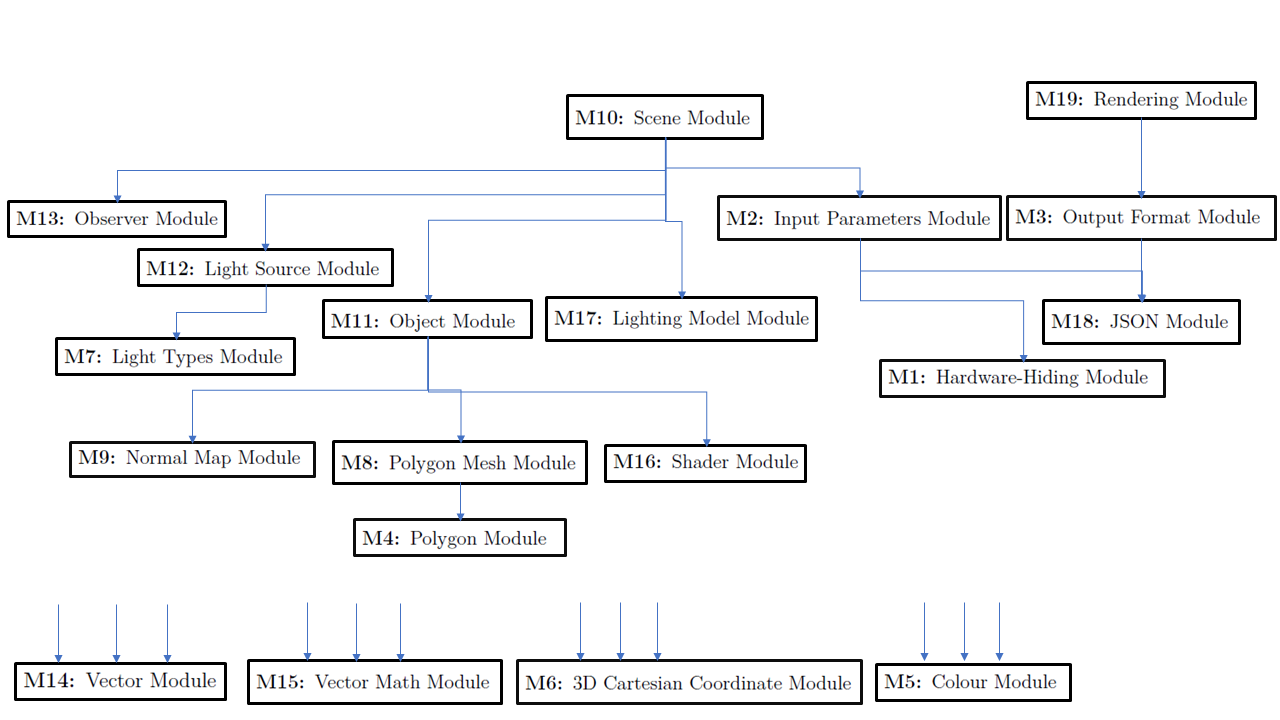
\includegraphics{mg-hierarchy}
%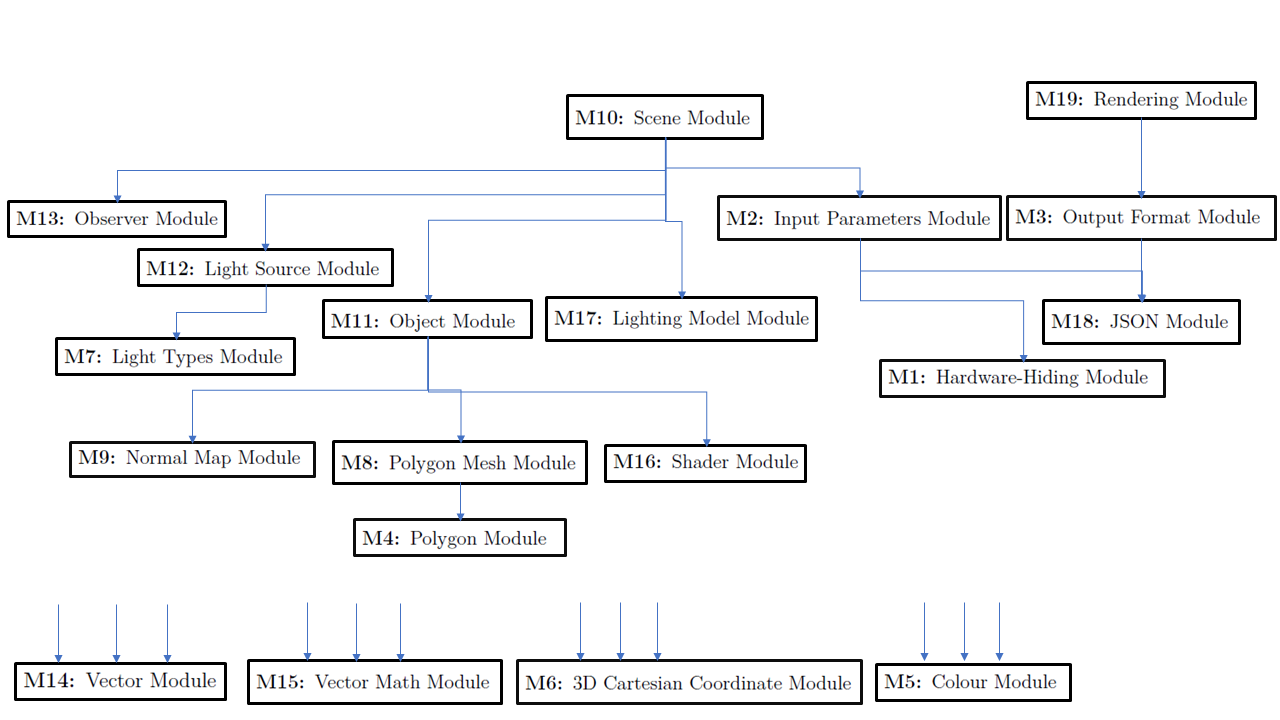
\includegraphics[width=0.7\textwidth]{./mg-hierarchy.png}
\caption{Use hierarchy among modules}
\label{FigUH}
\end{figure}

%\section*{References}

\bibliographystyle {plainnat}
\bibliography{../../refs/References}

\end{document}